\chapter{Kirchhoff Seismic Pre-Stack Depth Migration Application}
\graphicspath{{chapters/exp_kirchhoff/}}


The application computes the values of $A$ and $\tau$ for the coarse grid, interpolates the values of $A$ and $\tau$ for the fine grid then updates the image on the fine grid.

\section{Algorithms}

\subsection{Algorithm of the method}

The Algorithm \ref{alg:first_look} is raw.
There is no optimisation but it is quite simple.
It is a basis on which the other algorithms are founded.

\begin{algorithm}[h]
	\DontPrintSemicolon
	\SetAlgoVlined
	\caption{Kirchhoff Migration \label{alg:first_look}}
	\ForEach{trace $t_{S,R}$}{
		Read the source S and the receiver R from $t_{S,R}$. \;
		\ForEach{point P(x,y,z) of the image}{
			Compute the travel time $Ts$ between $S$ and $P$ (using Green functions)\;
			Compute the travel time $Tr$ between $P$ and $R$ (using Green functions)\;
			Compute the amplitude $A_{S,R}(x,y,z)$.\;
			$im(x,y,z)=im(x,y,z) + A_{S,R}(x,y,z) \cdot t_{S,R}(Ts + Tr)$
		}
	}
\end{algorithm}

\begin{algorithm}[h]
	\DontPrintSemicolon
	\SetAlgoVlined
	\caption{Kirchhoff Migration with coarse and fine grids\label{alg:kirchhoff_multigrids}}
	\ForEach{trace t}{
		\ForEach{(x, y, z) in the coarse grid CG}{
			r = extractR(t)\;
			s = extractS(t)\;
			CG(x, y, z).TS(s) = computeTravelTimeFromVelocityModel(s, x, y, z)\;
			CG(x, y, z).TR(r) = computeTravelTimeFromVelocityModel(r, x, y, z)\;
			CG(x, y, z).A(s,r) = computeAmplitude(s, r, x, y, z)\;
			\ForEach{(i, j, k) in the fine grid FG}{
				CG(x, y, z).FG(i, j, k).TS(s) = interpolateTime(i, j, k, CG(x, y, z).TS(s), CG(x + 1, y, z).TS(s), CG(x - 1, y, z).TS(s), CG(x, y + 1, z).TS(s), CG(x, y - 1, z).TS(s), CG(x, y, z + 1).TS(s), CG(x, y, z - 1).TS(s))\;
				CG(x, y, z).FG(i, j, k).TR(r) = interpolateTime(i, j, k, CG(x, y, z).TR(r), CG(x + 1, y, z).TR(r), CG(x - 1, y, z).TR(r), CG(x, y + 1, z).TR(r), CG(x, y - 1, z).TR(r), CG(x, y, z + 1).TR(r), CG(x, y, z - 1).TR(r))\;
				CG(x, y, z).FG(i, j, k).A(s,r) = interpolateAmplitude(i, j, k, CG(x, y, z).A(s,r), CG(x + 1, y, z).A(s,r), CG(x - 1, y, z).A(s,r), CG(x, y + 1, z).A(s,r), CG(x, y - 1, z). A(s,r), CG(x, y, z + 1).A(s,r), CG(x, y, z - 1).A(s,r))\;
				CG(x, y, z).FG(i, j, k).v += CG(x, y, z).FG(i, j, k).A(s, r) x ts,r(CG(x, y, z).FG(i, j, k).TS(s) + CG(x, y, z).FG(i, j, k).TR(r))\;
			}
		}
	}
\end{algorithm}

Algorithm \ref{alg:first_look} is computationally bound since the computation of the travel time between $S$ and $R$ through $P$ takes a long time.
Indeed, the travel time is computed by using Green functions which are heavy to compute from the initial velocity model.
In practice two optimisations are used : multi-grids and pre-computation of the Green functions.

Algorithm \ref{alg:kirchhoff_multigrids} illustrates the use of two grids.
In the multi-grids approach, the travel time is computed for the coarse grid then interpolated for the fine grid.
The travel time for each point of the fine grid is interpolated from the travel time computed for the coarse grid.


\begin{algorithm}[h]
	\DontPrintSemicolon
	\SetAlgoVlined
	\caption{Kirchhoff Migration with multi-grids and loading precomputed Green functions \label{alg:kirchhoff_mg+load}}
	\ForEach{trace t}{
		\ForEach{(x, y, z) in the coarse grid CG}{
			r = extractR(t)\;
			s = extractS(t)\;
			Gs = loadPrecomputedGreenFunc(s)\;
			Gr = loadPrecomputedGreenFunc(r)\;
			CG(x, y, z).TS(s) = computeTravelTimeFromGreenFunc(Gs, x, y, z)\;
			CG(x, y, z).TR(r) = computeTravelTimeFromGreenFunc(Gr, x, y, z)\;
			CG(x, y, z).A(s,r) = computeAmplitude(s, r, x, y, z)\;
			\ForEach{(i, j, k) in the fine grid FG}{
				CG(x, y, z).FG(i, j, k).TS(s) = interpolateTime(i, j, k, CG(x, y, z).TS(s), CG(x + 1, y, z).TS(s), CG(x - 1, y, z).TS(s), CG(x, y + 1, z).TS(s), CG(x, y - 1, z).TS(s), CG(x, y, z + 1).TS(s), CG(x, y, z - 1).TS(s))\;
				CG(x, y, z).FG(i, j, k).TR(r) = interpolateTime(i, j, k, CG(x, y, z).TR(r), CG(x + 1, y, z).TR(r), CG(x - 1, y, z).TR(r), CG(x, y + 1, z).TR(r), CG(x, y - 1, z).TR(r), CG(x, y, z + 1).TR(r), CG(x, y, z - 1).TR(r))\;
				CG(x, y, z).FG(i, j, k).A(s,r) = interpolateAmplitude(i, j, k, CG(x, y, z).A(s,r), CG(x + 1, y, z).A(s,r), CG(x - 1, y, z).A(s,r), CG(x, y + 1, z).A(s,r), CG(x, y - 1, z). A(s,r), CG(x, y, z + 1).A(s,r), CG(x, y, z - 1).A(s,r))\;
				CG(x, y, z).FG(i, j, k).v += CG(x, y, z).FG(i, j, k).A(s, r) x ts,r(CG(x, y, z).FG(i, j, k).TS(s) + CG(x, y, z).FG(i, j, k).TR(r))\;
			}
		}
	}
\end{algorithm}

Algorithm \ref{alg:kirchhoff_mg+load} shows the use of the two optimisations.
The two grids are used and the Green functions are loaded from the file system.

\subsection{Parallelism}
In the Kirchhoff Migration, only the output image is modified.
The traces and the Green functions are accessed only for reading.
Therefore, the update of the image by the contribution of a trace conditions the parallelism available.
Moreover, the traces are independent and the update of a point of the image depends only on the contribution of the trace.

It leans that \textbf{all the points can be updated at the same time by a trace}.
It also means that there is concurrency problems if a point is updated by two traces.
Actually, since the update is a sum, it is worth considering to create images for different sets of traces independently then reduce (sum) the different images into a final image.

From a computational point of view, traces can be treated in any order and points can be computed independently.
Several traces can be treated at the same time with reductions on the output images.
So there is a lot of available computational parallelism but there is also data to transfer between compute units and from the file system.
Moreover, creating several images to reduce them later also produces communications to reunite them into one.
In the case where the Green functions are precomputed, loading them into the memory can be an issue.
They take a lot of space on disk so it is expensive to load them several times.

Thus, scheduling those data movements can be a good alternative to find an efficient way to manage the data without having to communicate too much.
In order to better express the dependencies, the method is described as a graph of tasks.

\subsection{Task algorithm}

The algorithms are rewritten to allow the use of tasks.
Basically, functions were created and those functions will be the tasks that will be used.
The task algorithm is the Algorithm \ref{alg:kirchhoff_task} and the function associated can be found in the Algorithm \ref{alg:kirchhoff_task_def}.

\begin{algorithm}[h]
	\DontPrintSemicolon
	\SetAlgoVlined
	\caption{Task Kirchhoff Migration \label{alg:kirchhoff_task}}
	\ForEach{trace t}{
		\ForEach{(x, y, z) in the coarse grid CG}{
			r = extractR(t)\;
			s = extractS(t)\;
			Gs = loadPrecomputedGreenFunc(s)\;
			Gr = loadPrecomputedGreenFunc(r)\;
			CG(x, y, z).TS(s) = computeTravelTimeFromGreenFunc(Gs, x, y, z)\;
			CG(x, y, z).TR(r) = computeTravelTimeFromGreenFunc(Gr, x, y, z)\;
			CG(x, y, z).A(s,r) = computeAmplitude(s, r, x, y, z)\;
			updateFineGrid(CG(x, y, z), CG(x + 1, y, z).TS(s), CG(x - 1, y, z).TS(s), CG(x, y + 1, z).TS(s), CG(x, y - 1, z).TS(s), CG(x, y, z + 1).TS(s), CG(x, y, z - 1).TS(s), CG(x + 1, y, z).TR(r), CG(x - 1, y, z).TR(r), CG(x, y + 1, z).TR(r), CG(x, y - 1, z).TR(r), CG(x, y, z + 1).TR(r), CG(x, y, z - 1).TR(r), CG(x + 1, y, z).A(s,r), CG(x - 1, y, z).A(s,r), CG(x, y + 1, z).A(s,r), CG(x, y - 1, z). A(s,r), CG(x, y, z + 1).A(s,r), CG(x, y, z - 1).A(s,r))\;
		}
	}
\end{algorithm}

In Algorithm \ref{alg:kirchhoff_task}, the tasks on the blocks of the coarse grid for a given trace can be executed in parallel.

\begin{algorithm}[h]
	\DontPrintSemicolon
	\SetAlgoVlined
	\caption{Task definition for Kirchhoff Migration \label{alg:kirchhoff_task_def}}
	\SetKwProg{Fn}{Task}{is}{end}

	\Fn{updateFineGrid(B:current block:inout;\;
	TSu, TSb, TSr, TSl, TSf, TSh:TravelTime;in\;
	TRu, TRb, TRr, TRl, TRf, TRh:TravelTime;in\;
	TSu, TSb, TSr, TSl, TSf, TSh:Amplitude;in)}{
		\ForEach{(i, j, k) in the fine grid FG}{
			B.FG(i, j, k).TS(s) = interpolateTime(i, j, k, B.TS(s), TSu, TSb, TSr, TSl, TSf, TSh)\;
			B.FG(i, j, k).TR(r) = interpolateTime(i, j, k, B.TR(r), TRu, TRb, TRr, TRl, TRf, TRh)\;
			B.FG(i, j, k).A(s,r) = interpolateAmplitude(i, j, k, B.A(s,r), TSu, TSb, TSr, TSl, TSf, TSh)\;
			B.FG(i, j, k).v += B.FG(i, j, k).A(s, r) x ts,r(B.FG(i, j, k).TS(s) + B.FG(i, j, k).TR(r))\;
		}
	}
\end{algorithm}

In Algorithm \ref{alg:kirchhoff_task_def}, the loop on the elements of the fine grid can also be executed in parallel.
There is at least two level of parallelism.


\subsection{Use of GPUs}
This section aims to add the use of GPUs in the Kirchhoff migration.
GPUs are slower than CPUs but there a lot more computing unit in GPUs.
They are used to process huge amount of parallel operations and they are very useful to perform simple operations on huge amount of data.
Therefore, most of the operations inside the fine grid can be performed on GPU since the operations are the same on all the data.
Indeed, the operation is a linear combination of several arrays at the same point.

\subsection{Pre-fetching and spreading the data}
Since the main issue is the communications between the storage system where the Green functions are and the computing units inside the super-computer, a solution would be to pre-fetch the data.
The Green functions would be stored in a storage system closer of the computing unit and faster.
It is possible to efficiently predict which Green function will be needed by the program when the source and the receiver of the trace are loaded.

Moreover, two block side by side share the Green functions at their frontier.
That means the same Green functions are loaded several times in a short amount of time from the file system.
The bandwidth between the file system and the computing unit is generally lower than the one between two nodes of the super-computer so use them will be more efficient.
To do so, the pre-fetcher will be modified to become aware of the tasks that uses the Green functions.
Then, if the Green function a task may want is still loaded in another task, the task using the Green function will send it to the task that also need it.
It will reduce the communications to the file system containing the Green functions and so, make the whole process faster.

To go further, a computing node of the super-computer may be able to store some of the Green functions even if it does not use them in order to provide them to the other nodes as long as possible.

\section{2D Implementations}

At the moment, the application will be simplified with $A=1$.
This application is available at \url{https://bitbucket.org/jgurhem/kirchhoffmigration/src/master/}.

\subsection{C, A=1}

The application is divided in several parts.
An application generates a trace, another one adds the propagation time to a trace by interpolating the travel times generated from a third one.
The last application make the migration from the trace with the travel time by interpolating the travel time at a finer grain than the one given in input.
It can take a trace file as input or a text file containing a list of trace files.

Figure \ref{fig:kirchhoff_trace} gives an example of a generated trace used to test the 2D application with these simplifications.
Figure \ref{fig:kirchhoff_pt} is a plot of the propagation times to make the round trip from the source point located at (1000,0), each point of the figure and the receiver located at (1000, 0) in a uniform middle.
Figure \ref{fig:kirchhoff_image} is the migrated image produced by the Kirchhoff migration with the trace of Figure \ref{fig:kirchhoff_trace} taken at several different source locations (the source and the receiver are located at the same place).


\begin{figure}[H]
	\centering
	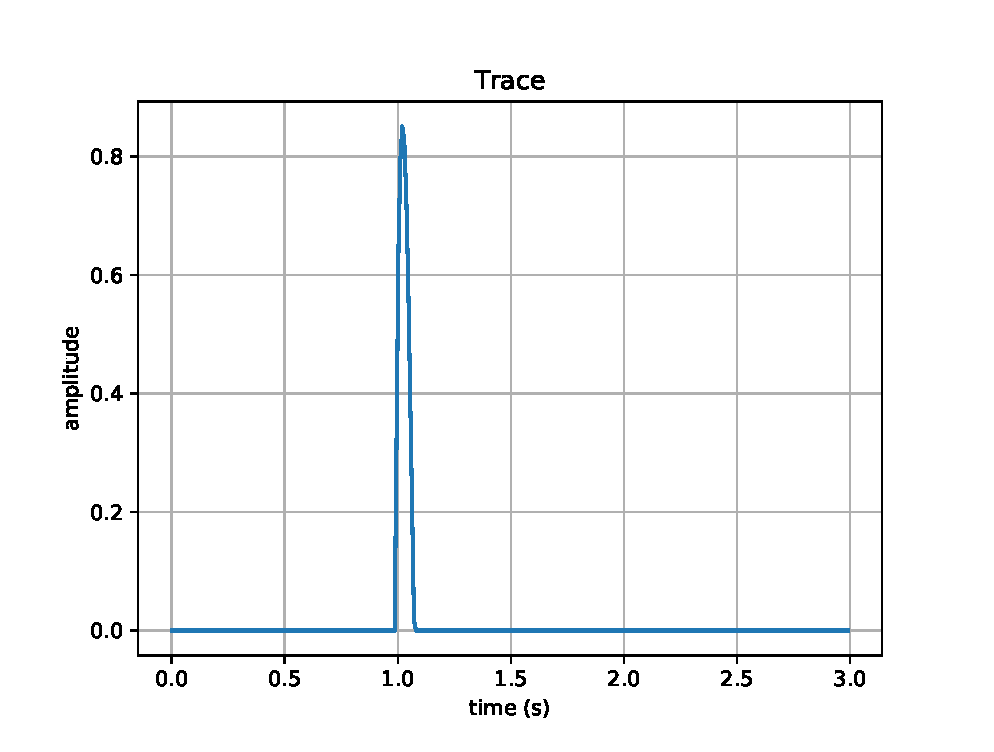
\includegraphics[scale=0.65]{trace}
	\caption{Trace example\label{fig:kirchhoff_trace}}
\end{figure}

\begin{figure}[H]
	\centering
	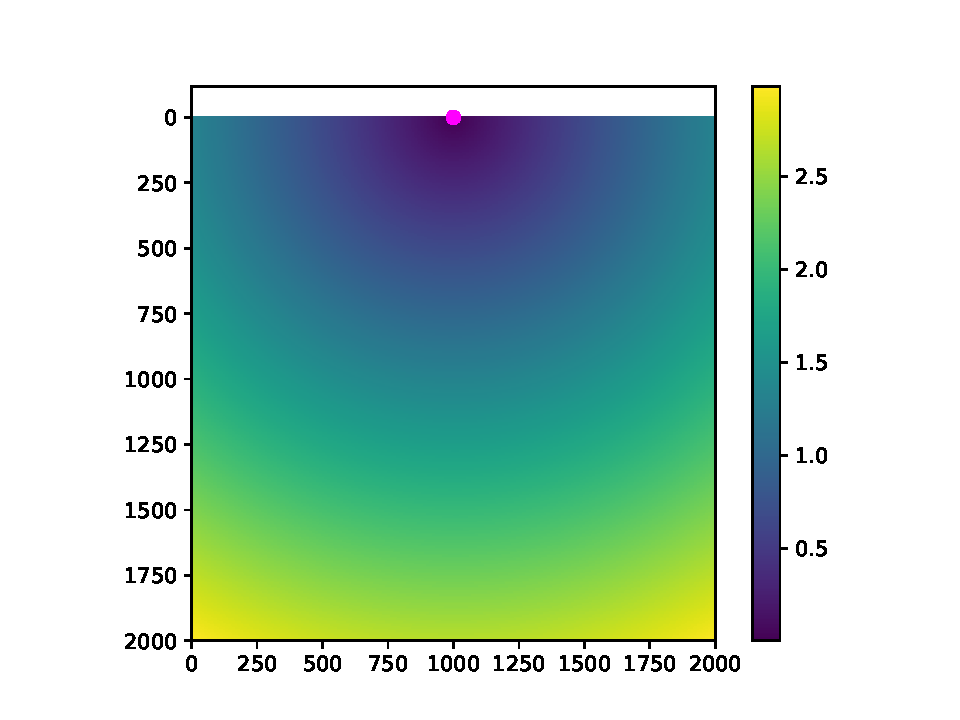
\includegraphics{trace1000ppt.pdf}
	\caption{Propagation times for a source and receiver at the same place\label{fig:kirchhoff_pt}}
\end{figure}

\begin{figure}[H]
	\centering
	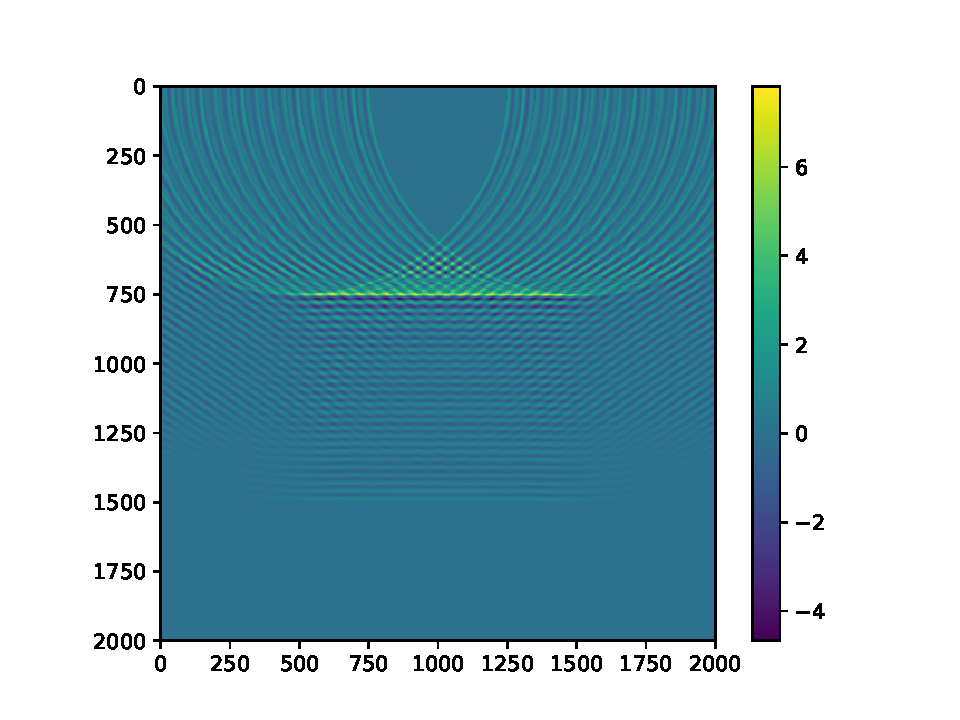
\includegraphics{img.pdf}
	\caption{Image obtained from a migrated trace\label{fig:kirchhoff_image}}
\end{figure}

\subsection{YML}
Here is examples of what the YML graph of the Kirchhoff migration would look like.
It shows the main application and the abstract of the Image component.

\begin{lstlisting}[tabsize=3, frame=single, basicstyle=\small\ttfamily, title=YML application]
<?xml version="1.0"?>
<application name="Kirchhoff">
<description> Kirchhoff method
</description>
<graph>

T:=100; #number of traces
X:=10; Y:=5; Z:=10; Xp:=10; Yp:=10; Zp:=10;

par(t:=1;T)
do
	compute Read(t,R,S)
	par(x:=1;X)(y:=1;Y)(z:=1;Z)
	do
		compute Load(S,Gs,R,Gr,B[x][y][z],Tb,Tt)
		if(|Tb-Ts|<0.01) then
			par(xp:=1;Xp)(yp:=1;Yp)(zp:=1;Zp)
			do
				compute Image(t,S,Gs,R,Gr,B[x][y][z],img[xp][yp][zp])
			enddo
		endif

	enddo
enddo
</graph>
</application>
\end{lstlisting}

The application contains the calls for the components, then they will make the different tasks on the data : loading, computing and generation of the image.

\begin{lstlisting}[tabsize=5, frame=single, basicstyle=\small\ttfamily, title=Abstract of Image task]
<?xml version="1.0" ?>
<component
	type="abstract"
	name="Image"
	description="Abstract of the Image task" >
<params>
	<param name="t" type="Trace" mode="in" />
	<param name="S" type="Source" mode="in" />
	<param name="Gs" type="Green" mode="in" />
	<param name="R" type="Receiver" mode="in" />
	<param name="Gs" type="Green" mode="in" />
	<param name="B" type="Block" mode="in" />
	<param name="img" type="Image" mode="inout" />
</params>
</component>
\end{lstlisting}

\begin{lstlisting}[tabsize=5, frame=single, basicstyle=\small\ttfamily, title=Abstract of Read task]
<?xml version="1.0" ?>
<component
	type="abstract"
	name="Read"
	description="Abstract of the Read task" >
<params>
	<param name="t" type="Trace" mode="in" />
	<param name="S" type="Source" mode="out" />
	<param name="R" type="Receiver" mode="out" />
</params>
</component>
\end{lstlisting}

\begin{lstlisting}[tabsize=5, frame=single, basicstyle=\small\ttfamily, title=Abstract of Load task]
<?xml version="1.0" ?>
<component
	type="abstract"
	name="Load"
	description="Abstract of the Load task" >
<params>
	<param name="S" type="Source" mode="in" />
	<param name="Gs" type="Green" mode="out" />
	<param name="R" type="Receiver" mode="in" />
	<param name="Gs" type="Green" mode="out" />
	<param name="B" type="Block" mode="in" />
	<param name="Tb" type="float" mode="in" />
	<param name="Tt" type="float" mode="in" />
</params>
</component>
\end{lstlisting}

The abstract components contain all the informations about the data transfer and define the parameters of the component.
With these data, YML is able to manage efficiently the data movements through the network and optimize the communications.

The implementation components contain the code executed during the call of the component.
There is no component implemented to make the Kirchhoff migration since the purpose is not to make a new program but propose new algorithms.


\section{2D Numerical Experiments}